\documentclass[a4paper,12pt, titlepage]{article}
\usepackage[finnish]{babel} %suomenkielinen tavutus
\usepackage[T1]{fontenc} %skanditavutus
\usepackage[utf8]{inputenc}        	% skandit utf-8 koodauksella
%\usepackage[ansinew]{inputenc}        	% skandit utf-8 koodauksella, kokeile tata, jos utf-8 ylla ei toimi.

\usepackage{graphicx}
\usepackage{pdfpages}
\usepackage{hyperref}
\usepackage{tabularx}
\usepackage{geometry}
 \geometry{
 a4paper,
 total={170mm,257mm},
 left=20mm,
 top=20mm,
 }

\linespread{1.24} %rivivali 1.5
\sloppy % Vahentaa tavutuksen tarvetta, "leventamalla" rivin keskella olevia valilyönteja.


\title{Helpperin arkkitehtuuri}
\author{ Maiju Airosmaa \\ Kalle Hiljanen \\
Outi Jussila \\ Eetu Mattila \\ Johanna Vehniäinen \\[1cm] Ohjelmiston arkkitehtuuridokumentaatio \\ Helsingin yliopisto}
\date{Toukokuu 2016}

\begin{document}

\maketitle

\tableofcontents
\newpage

\section{Järjestelmän yleiskuvaus ja rakenne}
\noindent
Sovellus on kehitetty käyttämällä Ruby on Railsia. Käytössä on Rubyn versio 2.3.1 ja Railsin versio 4.2.6. Näkymien toiminnallisuuksien toteutuksessa on käytetty myös jonkun verran Javascriptiä. Data selaimen ja kontrollereiden välillä on välitetty osittain JSON-muodossa.
\newline
\newline
Ohjelmiston arkkitehtuuri noudattaa MVC-mallia eli keskustelu näkymien ja mallien sekä tietokannan välillä tapahtuu kontrollereiden kautta.

\section{Relaatiotietokantakaavio}

\noindent\makebox[\textwidth]{%
\begin{tabularx}{1.1\textwidth}{XX}
  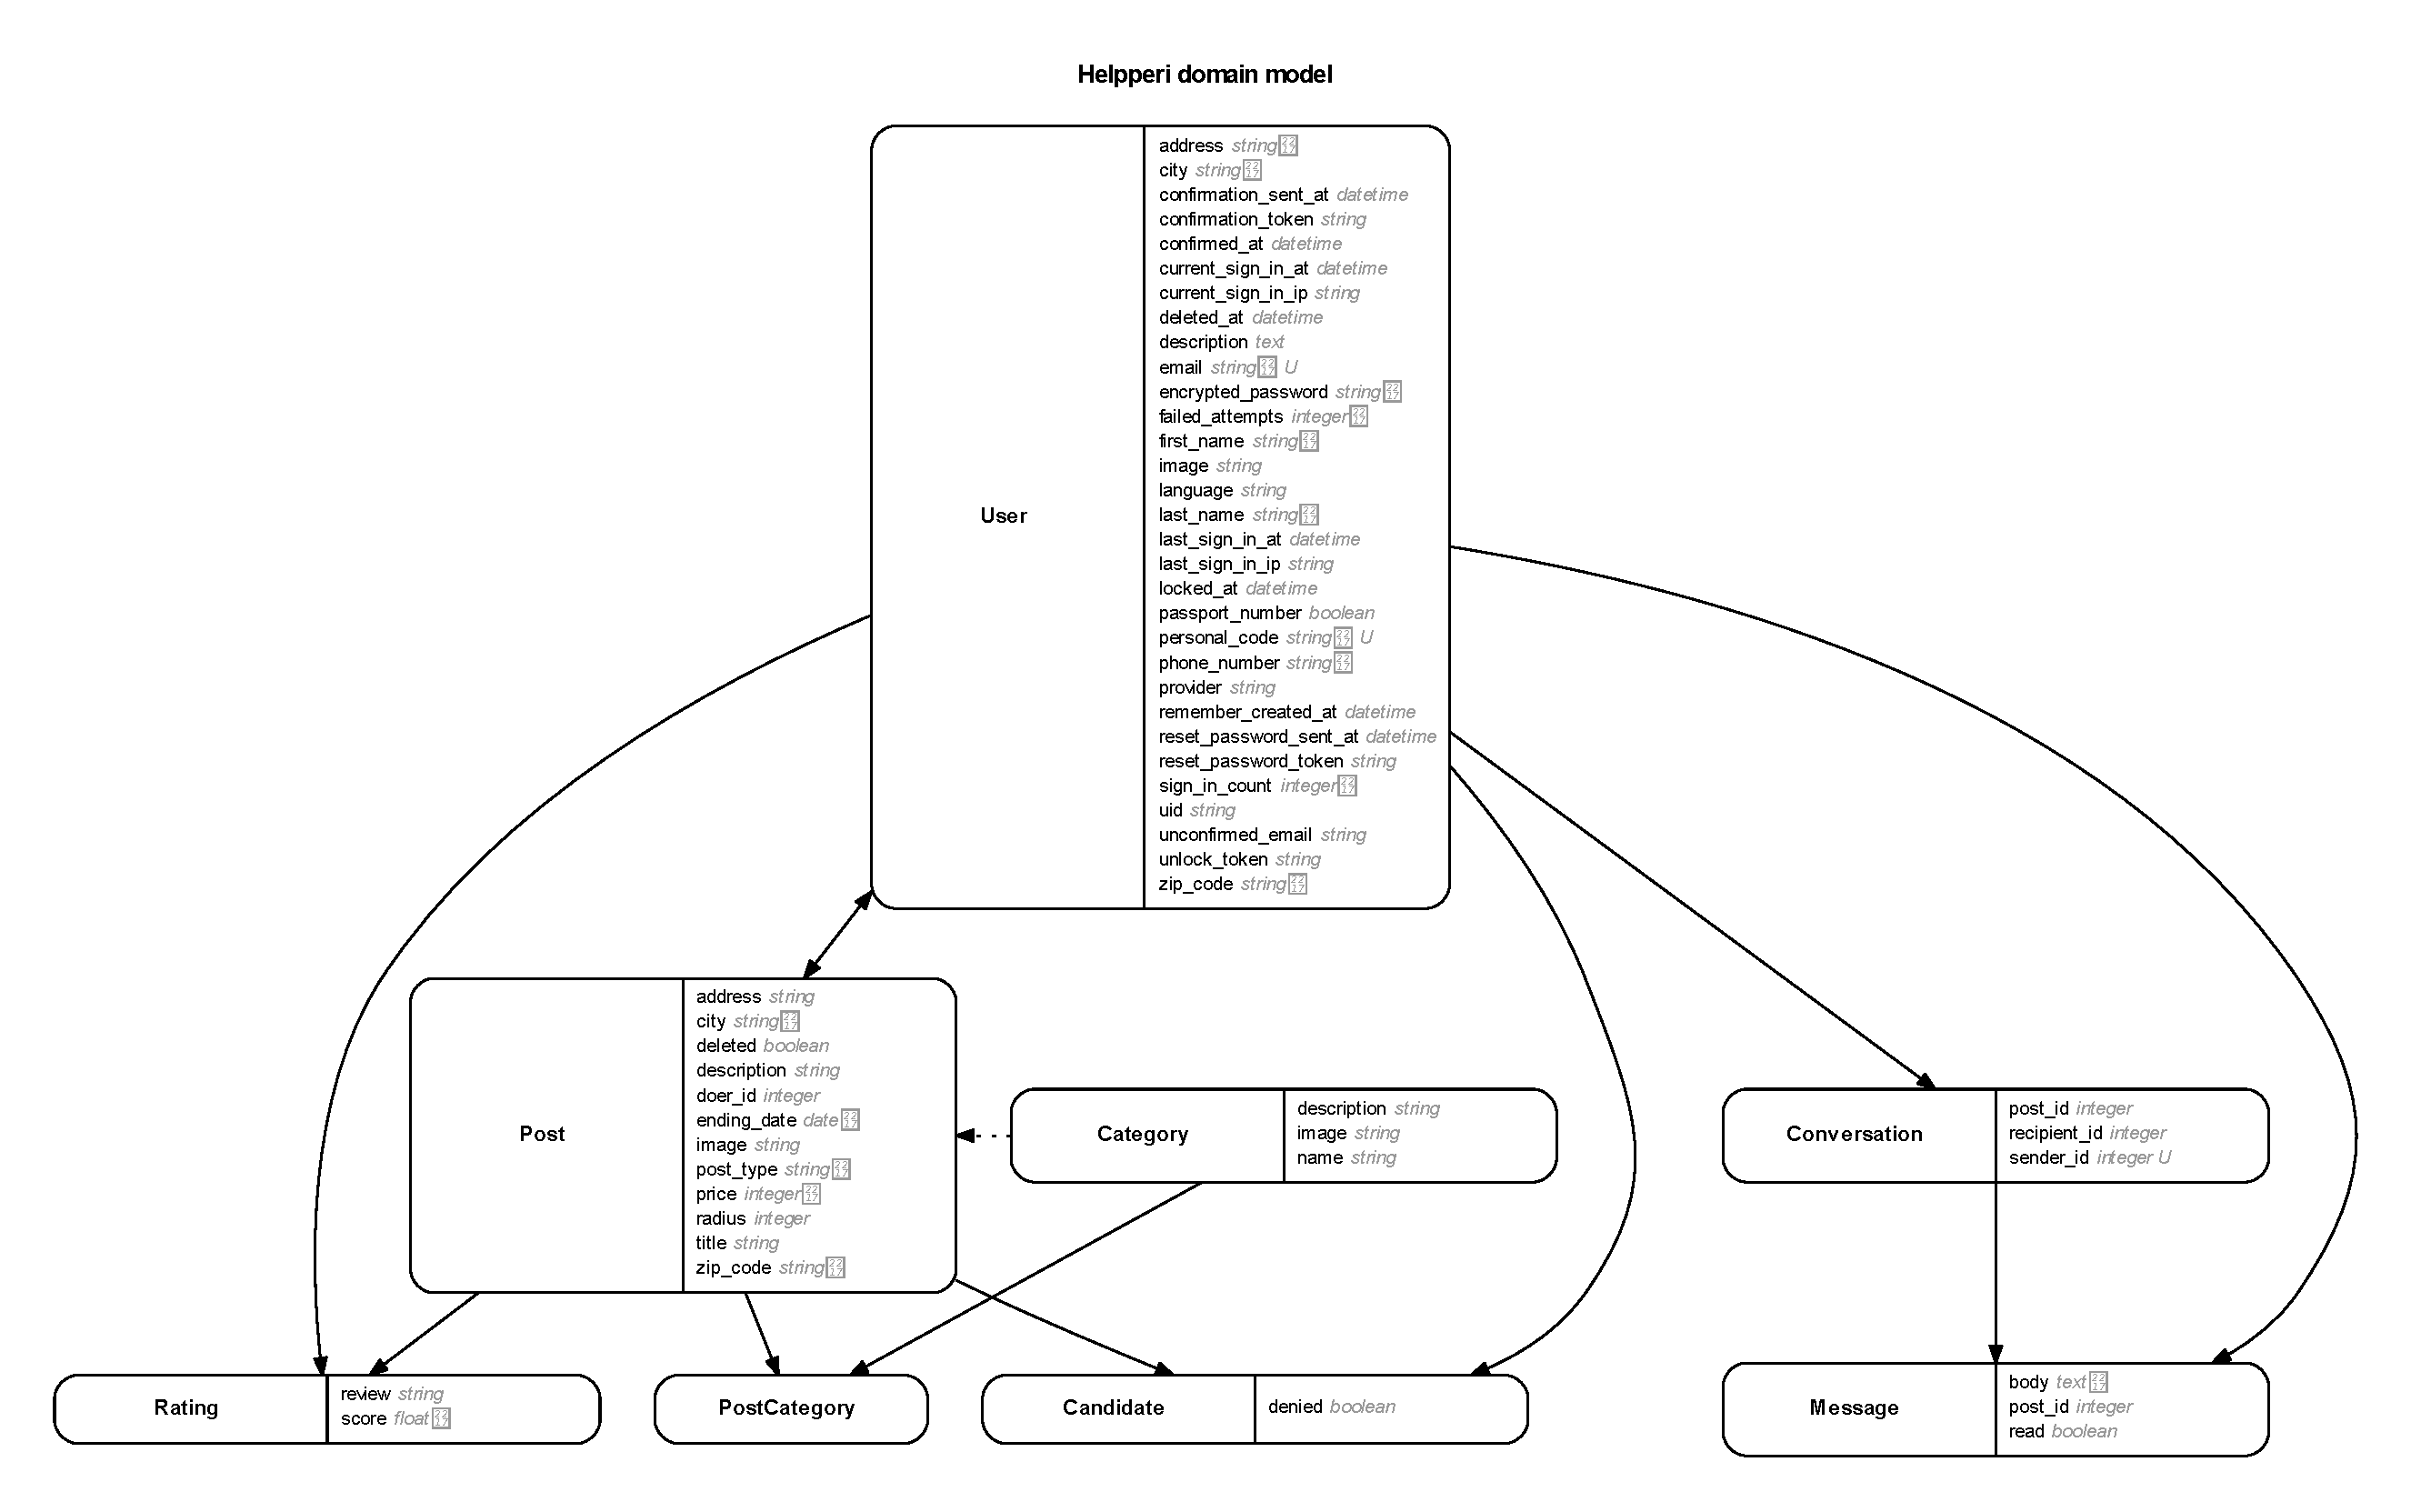
\includegraphics[width=190mm]{kaavio}
\end{tabularx}}
\newline
\newline
\newline
\newline
Tietokannassa on yhteensä 8 taulua. Lisäksi kaksi PublicActivity- ja Unread-gemin luomia tauluja, jotka on jätetty selkeyden vuoksi pois kaaviosta.
\newline
Käyttäjällä (User) voi olla useita ilmoituksia (Post), arvosteluja (Rating), keskusteluja (Conversation) ja viestejä (Message). Arvosteluissa käyttäjä on joko arvioituna (revieved\_id) tai arvioijana (reviewer\_id).
\newline
Ilmoitukseen liittyy yksi käyttäjä ilmoittajana (user\_id) ja voi liittyä yksi käyttäjä suorittajana (doer\_id). Lisäksi ilmoituksella voi olla useita kiinnostuneita käyttäjiä Candidate-taulun kautta. Ilmoitukseen liittyy maksimissaan kaksi arvostelua, jotka kuuluvat ilmoittajalle ja suorittajalle. Ilmoitus muuttuu suoritetuksi (scope rated), kun arvosteluja on kaksi. Ilmoitus kuuluu yhdelle tai useammalle kategorialle (Category) välitaulun (PostCategory) kautta.
\newline
Keskusteluun liittyy kaksi käyttäjää (sender\_id, recipient\_id). Lisäksi keskustelu voi liittyä yhteen ilmoitukseen. Kahden käyttäjän välillä voi olla vain yksi keskustelu, joka ei liity mihinkään ilmoitukseen, ja lisäksi heidän välillään voi olla ilmoituskohtaisia keskusteluja. Keskusteluun liittyy useita viestejä. Viestit liittyvät keskustelun kautta ilmoituksiin. Viestien attribuutti post\_id ei ole käytössä. 

\section{Liitteet}

GitHub:
\url{https://github.com/xjoxjox/helpperi}

\end{document}
